\documentclass{article}
\usepackage{amsmath}
\usepackage{graphicx}
\usepackage{float}
\begin{document}
\section{Overview}
The largest and bulkiest device on any electrical vehicle is the battery.
Dense energy storage is a difficult task, and batteries are a must for almost all devices.
\section{Capacity}
The larger the capacity of a battery network, the larger, heavier, and more expensive the battery network becomes.
The use case of the system needs to be considered for choosing a capacity.
Capacitance is normally measured in Amp-Hours, or how many hours a battery can supply the rated current at the nominal voltage of the battery.

When specifying capacity for an electric vehicle, two factors are going to be needed:
\begin{itemize}
    \item Range
    \item Efficiency
\end{itemize}
The nominal range will be determined by the expected average daily usage, and the specified charge frequency. 
The value given for charge frequency will be once a week.
The daily usage will be a round trip from Josephine butler to the engineering department on the science site each way this is ~1.3km, this is shown in Fig. \ref{fig:route}.
\begin{figure}[H]
    \centering
    \scalebox{0.5}{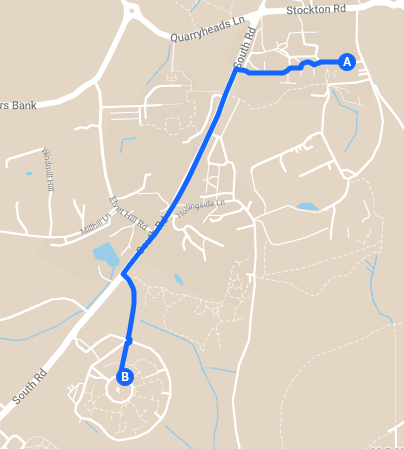
\includegraphics{./RouteAnalysis/Route.png}}
    \caption{Nominal daily route}
    \label{fig:route}
\end{figure}
Due to Durhams geographical features and the relatively small distances involved, the range needs to account for the elevation changes over the trip.
The exact elevation change can be seen in \ref{fig:route_el}, with the gradients of this data in \ref{fig:route_grad}.
This data is taken from GPS public databases via https://www.gpsvisualizer.com/elevation.
The routes were made using google maps - exported to GPS route format.
\begin{figure}[H]
    \centering
    \scalebox{0.5}{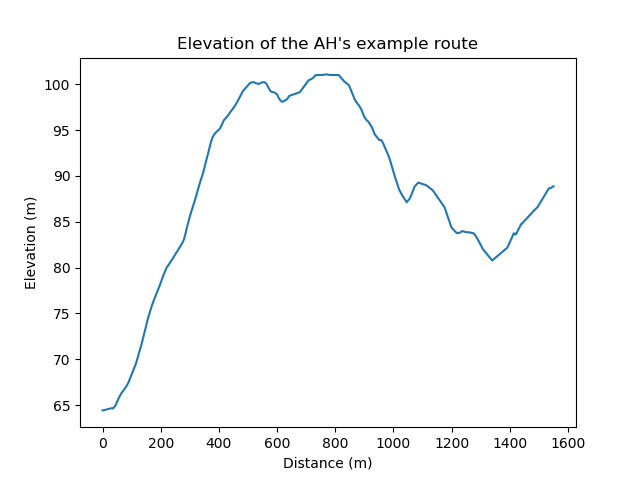
\includegraphics{./RouteAnalysis/elevation.png}}
    \caption{Gradient of route}
    \label{fig:route_el}
\end{figure}
Fig. \ref{fig:route_el} shows the elevation through the route, with south road easily identifiable. 
\begin{figure}[H]
    \centering
    \scalebox{0.5}{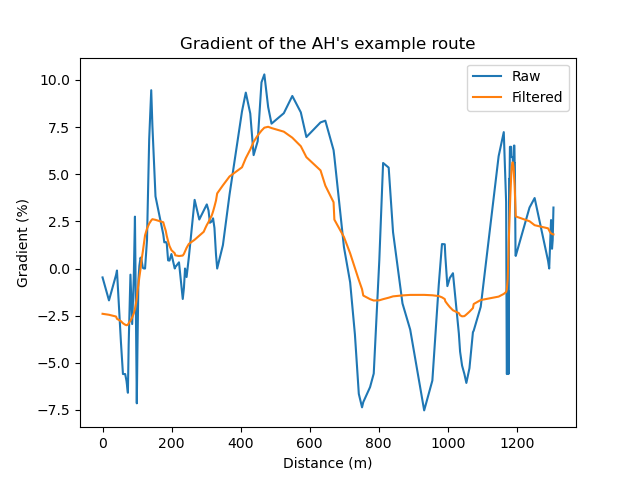
\includegraphics{./RouteAnalysis/grad.png}}
    \caption{Elevation of route}
    \label{fig:route_grad}
\end{figure}
There is a total of 41 meters uphill, and 16 meters downhill when going towards butler.
The effect of the height change on the capacity will be non negligible.
Roughly 33kJ more energy will be needed with a perfect system.

Rough power estimates: 
10 watt hours per mile - electric bike
12 watt hours per journey (flat)

\section{Charging}
Battery charging is difficult, specific charging circuits are needed for most modern high density batteries.
When trying to charge lots of batteries quickly a large amount of heat is generated, which needs to be considered in the design stage.
Large modern batteries can also be very dangerous - and this is amplified when charging, so care needs to be taken that the design isn't a health hazard.
\end{document}
